\subsection{Candidate-Pool Expansion for Zero-Capacity Cells}
\label{sec:mip_pool_expansion}

A pool that is feasible and cell-complete at the level of the modelled
attributes need not have capacity at the level of a specific zone. For a given
zone a control-table cell can require more records than the pool supplies, and
in the limiting case no household in the zone's candidate pool carries the cell
at all. This \emph{zero-capacity cell} is a support gap rather than a data
error, and reweighting cannot repair it: iterative proportional updating adjusts
the weights of existing records but cannot create a record with an unobserved
combination. Candidate-pool expansion therefore adds the smallest set of
rule-feasible records needed to make such cells selectable, and leaves partial
shortfalls---cells with positive but insufficient capacity---to the zone fitter,
which can replicate a candidate within its own replication limit.

\paragraph{Constructing candidates.}
For each zero-capacity cell the module draws a donor record from the census
microdata that carries the required category and grafts the donor's person
profile into a real household ``shell'' from the same region that has a vacancy
in the matching household role. If the grafted profile conflicts with the
shell's dwelling terms or with the structural rules, a small repair step
substitutes the closest rule-feasible profile; candidates that still fail the
structural checks are discarded rather than patched. The household-level fields
are fixed to the shell, so every candidate is a complete, internally consistent
household. For the few attributes that lie outside the person-level rule set and
have no person-level repair, the module instead copies a whole observed donor
household, which is feasible by construction.

\paragraph{Selecting candidates.}
The candidates are selected together rather than one cell at a time. A single
selection is chosen to cover every zero-capacity cell for which a feasible
candidate exists, using as few added households as possible and---among
selections that achieve the same coverage---keeping the added set's aggregate
composition close to the zone's marginal totals. Coverage is the priority: a
cell with no feasible candidate anywhere cannot make the problem infeasible and
is reported instead of forced, and because each added household is penalised, the
selection stops once every sourceable cell is covered. In practice the coverage
objective dominates, so the marginal-matching term acts as a tie-breaker among
equally good coverings rather than as a fit to the zone's full distribution---the latter is the object of the zone fitter. The two optimisation programs (a
per-candidate repair and the selection program) are stated in
Appendix~\ref{sec:pool_expansion_audit}; \cref{fig:mip-expansion-process}
traces the four stages from the cell audit to the appended households.

% Figure 2: visual representation of MIP candidate-pool expansion.
\begin{figure}[htbp]
\centering
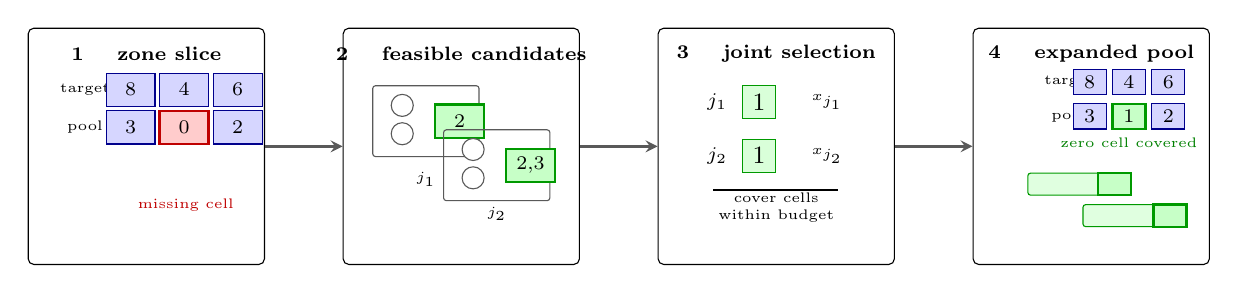
\begin{tikzpicture}[
  >=stealth,
  every node/.style={font=\small},
  panel/.style={draw, rounded corners=2pt, inner sep=5pt},
  title/.style={font=\scriptsize\bfseries, align=center},
  cell/.style={draw, minimum width=0.62cm, minimum height=0.42cm,
               inner sep=0pt, align=center, font=\scriptsize},
  have/.style={cell, fill=blue!16, draw=blue!55!black},
  zero/.style={cell, fill=red!20, draw=red!75!black, line width=0.9pt},
  add/.style={cell, fill=green!22, draw=green!60!black, line width=0.8pt},
  person/.style={circle, draw=black!65, fill=white, minimum size=0.28cm,
                 inner sep=0pt},
  shell/.style={draw=black!65, rounded corners=1pt, minimum width=1.35cm,
                minimum height=0.9cm, inner sep=2pt},
  arrow/.style={->, line width=0.9pt, draw=black!65}
]

% 1. A zone-specific zero-capacity cell.
\node[panel, minimum width=3.0cm, minimum height=3.0cm] (audit) at (0,0) {};
\node[title] at (0,1.18) {1 \quad zone slice};
\node[font=\tiny] at (-0.78,0.72) {target};
\node[font=\tiny] at (-0.78,0.24) {pool};
\foreach \x/\target/\cap in {-0.20/8/3,0.48/4/0,1.16/6/2} {
  \node[have] at (\x,0.72) {\target};
  \ifnum\cap=0
    \node[zero] at (\x,0.24) {\cap};
  \else
    \node[have] at (\x,0.24) {\cap};
  \fi
}
\node[font=\tiny, text=red!75!black] at (0.50,-0.75) {missing cell};

% 2. Feasible donor-shell household candidates.
\node[panel, minimum width=3.0cm, minimum height=3.0cm] (candidates) at (4.0,0) {};
\node[title] at (4.0,1.18) {2 \quad feasible candidates};
\node[shell] (h1) at (3.55,0.32) {};
\node[person] at (3.25,0.52) {};
\node[person] at (3.25,0.16) {};
\node[add] at (3.98,0.32) {2};
\node[font=\tiny] at (3.55,-0.42) {$j_1$};
\node[shell] (h2) at (4.45,-0.24) {};
\node[person] at (4.15,-0.04) {};
\node[person] at (4.15,-0.40) {};
\node[add] at (4.88,-0.24) {2,3};
\node[font=\tiny] at (4.45,-0.86) {$j_2$};

% 3. MIP chooses a covering set.
\node[panel, minimum width=3.0cm, minimum height=3.0cm] (select) at (8.0,0) {};
\node[title] at (8.0,1.18) {3 \quad joint selection};
\node[font=\scriptsize] at (7.25,0.56) {$j_1$};
\node[font=\scriptsize] at (7.25,-0.12) {$j_2$};
\node[draw=green!60!black, fill=green!15, minimum width=0.42cm,
      minimum height=0.42cm, inner sep=0pt] at (7.78,0.56) {$1$};
\node[draw=green!60!black, fill=green!15, minimum width=0.42cm,
      minimum height=0.42cm, inner sep=0pt] at (7.78,-0.12) {$1$};
\node[font=\tiny] at (8.65,0.56) {$x_{j_1}$};
\node[font=\tiny] at (8.65,-0.12) {$x_{j_2}$};
\draw[thick] (7.20,-0.55) -- (8.78,-0.55);
\node[font=\tiny, align=center] at (8.0,-0.78) {cover cells\\within budget};

% 4. Original pool plus appended households; the zero cell is now supported.
\node[panel, minimum width=3.0cm, minimum height=3.0cm] (expanded) at (12.0,0) {};
\node[title] at (12.0,1.18) {4 \quad expanded pool};
\node[font=\tiny] at (11.72,0.82) {target};
\node[font=\tiny] at (11.72,0.38) {pool};
\foreach \x/\target/\cap in {11.98/8/3,12.48/4/1,12.98/6/2} {
  \node[have, minimum width=0.42cm, minimum height=0.32cm] at (\x,0.82) {\target};
  \ifnum\cap=1
    \node[add, minimum width=0.42cm, minimum height=0.32cm] at (\x,0.38) {\cap};
  \else
    \node[have, minimum width=0.42cm, minimum height=0.32cm] at (\x,0.38) {\cap};
  \fi
}
\node[font=\tiny, text=green!50!black] at (12.48,0.04) {zero cell covered};
\node[shell, draw=green!60!black, fill=green!12, minimum width=1.05cm,
      minimum height=0.28cm, inner sep=0pt] at (11.72,-0.48) {};
\node[add, minimum width=0.42cm, minimum height=0.28cm] at (12.30,-0.48) {};
\node[shell, draw=green!60!black, fill=green!12, minimum width=1.05cm,
      minimum height=0.28cm, inner sep=0pt] at (12.42,-0.88) {};
\node[add, minimum width=0.42cm, minimum height=0.28cm] at (13.00,-0.88) {};

\draw[arrow] (audit.east) -- (candidates.west);
\draw[arrow] (candidates.east) -- (select.west);
\draw[arrow] (select.east) -- (expanded.west);

\end{tikzpicture}
\caption{Visual distinction between global CP construction and zone-specific MIP pool
expansion. The zone slice begins with a red zero-capacity cell: its target is positive,
but no current pool record can supply it. Feasible donor--shell households are represented
as candidate cards, with the colored tags showing the cells each household covers. The
joint MIP marks the candidates selected together under coverage and budget constraints.
The final panel shows the original pool rows retained and the selected households appended
in green. This enlarges candidate support before SA, IPU, or MIP fitting; it does not
construct the final zone population.}
\label{fig:mip-expansion-process}
\end{figure}


\paragraph{Scope.}
The step is deliberately \emph{not} required to close the zone's full deficit.
That deficit is often tens of thousands of persons, whereas the candidate pool
is a five-per-cent microsample and the added set is a handful of households;
requiring the pool to reproduce the shortfall would either be infeasible or
force it to replicate the census many times over, which is the fitter's role,
not the pool's. What expansion guarantees is weaker and sufficient: every zero
cell with a feasible candidate becomes selectable, with the fewest rule-feasible
additions, and the fitting stage that follows decides which candidates are used.

\paragraph{Demonstration.}
On ten SA2 zones the mechanism identified 123 zero-capacity cells among 146
deficient cells (the remaining 23 were partial shortfalls). It produced feasible
candidates for 70 of the 73 cells that were sourceable, and the selection covered
all 70, adding 14 households (18 persons) in total---one or two households per
zone. Coverage is therefore achieved without forcing the pool to reproduce the
shortfall, every added record satisfies the shared structural constraints, and
the expanded pool introduces no new constraint violations. The 53 uncovered cells
are not donor shortages but categories the data cannot source: 40 lie in four
codes absent from the census extract and ten are a padding code, leaving three
cells for which no feasible donor--shell candidate was found. The per-zone result
and the formulation are in Appendix~\ref{sec:pool_expansion_audit}.

\begin{figure}[htbp]
\centering
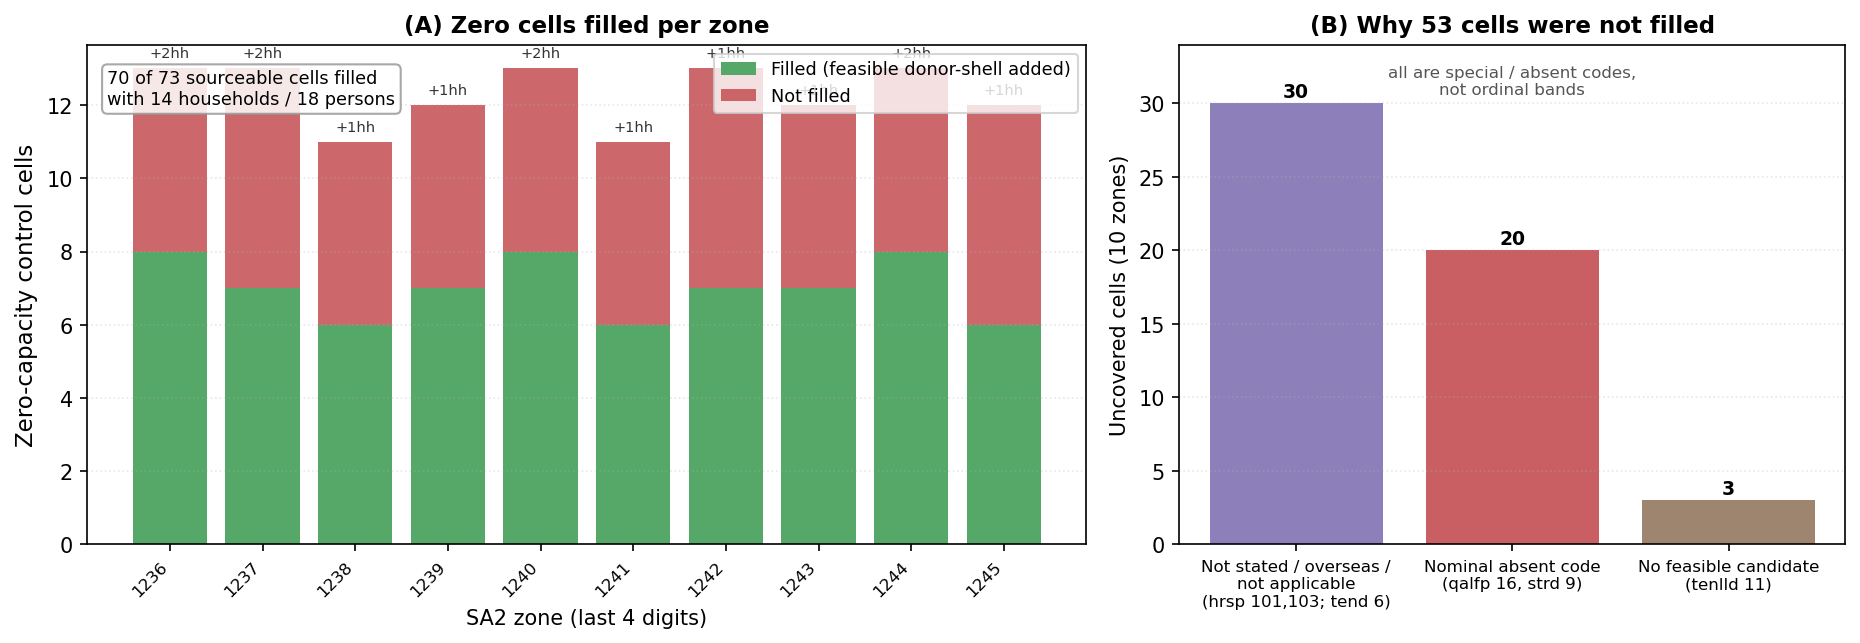
\includegraphics[width=0.95\linewidth]{zero_cell_coverage.png}
\caption{Candidate-pool expansion on ten SA2 zones. \textbf{(A)} For each zone,
the zero-capacity control cells that the expansion filled by adding a feasible
donor--shell household (green) versus those it left unfilled (red); the
annotation gives the number of households the selection added. All 70 sourceable
cells were filled with 14 households (18 persons). \textbf{(B)} The 53 unfilled
cells by reason. All but three are \emph{special or absent codes} rather than
sourceable bands: the \texttt{hrsp} cells are the ``not stated'' (101) and
``overseas visitor'' (103) codes and \texttt{tend:6} is a not-applicable padding
code, while \texttt{qalfp:16} and \texttt{strd:9} are nominal categories absent
from the census extract; only the three \texttt{tenlld:11} cells had a positive
target with no feasible candidate. Genuinely \emph{ordinal} shortfalls---an
applicable income, hours, or qualification-level band with no donor---are instead
filled by borrowing the nearest applicable band and shifting the value to the
target, restricted to the employment/age-applicable range (children and
not-applicable persons are never shifted into an ordinal band) and re-checked
against the individual and household rules.}
\label{fig:zero_cell_coverage}
\end{figure}
\FloatBarrier
